\documentclass[conference]{IEEEtran}
\pagestyle{plain}
\hyphenation{op-tical net-works semi-conduc-tor}

\usepackage{todonotes}
\usepackage[tight,footnotesize]{subfigure}

\usepackage{hyperref}
\hypersetup{
	breaklinks,
    pdfpagemode={UseOutlines},
    bookmarksopen,
    pdfstartview={FitH},
    colorlinks,
    linkcolor={blue},
    citecolor={red},
    urlcolor={blue}
}


\begin{document}
\title{
Distributed Security Risks and Opportunities \\
in the %\\
W3C Web of Things
}
\author{
  \IEEEauthorblockN{Michael McCool}
  \IEEEauthorblockA{Intel Corporation\\
                    michael.mccool@intel.com}
\and
  \IEEEauthorblockN{Elena Reshetova}
  \IEEEauthorblockA{Intel Corporation\\
                    elena.reshetova@intel.com}
}

\IEEEoverridecommandlockouts
\makeatletter\def\@IEEEpubidpullup{9\baselineskip}\makeatother
\IEEEpubid{\parbox{\columnwidth}{Permission to freely reproduce all or part
    of this paper for noncommercial purposes is granted provided that
    copies bear this notice and the full citation on the first
    page. Reproduction for commercial purposes is strictly prohibited
    without the prior written consent of the Internet Society, the
    first-named author (for reproduction of an entire paper only), and
    the author's employer if the paper was prepared within the scope
    of employment.  \\
    NDSS '18, 18-21 February 2018, San Diego, CA, USA\\
    Copyright 2018 Internet Society, ISBN 1-1891562-49-5\\
    http://dx.doi.org/10.14722/ndss.2018.23008
}
\hspace{\columnsep}\makebox[\columnwidth]{}}
\maketitle

\begin{abstract}
The W3C Web of Things (WoT) WG has been developing an interoperability standard for IoT devices that includes as
its main deliverable a ``Thing Description'': a standardized representation for the metadata of an 
IoT device, including in particular a description of its network interface,
but also allowing for multiple levels of semantic annotation.
The WoT Thing Description supports a descriptive (as opposed to prescriptive) approach to interoperability.
The provision of rich descriptive metadata has at least five major implications for security.
First, the need for local links and, more generally, disconnected and segmented networks
       in IoT raises several practical considerations regarding what metadata should be provided.
Second, metadata allows for system-wide vulnerability analysis, 
       which can be both a risk and an opportunity.
Third, metadata can enable end-to-end security in multistandards networks,
       avoiding exposing unencrypted data within bridges otherwise needed for adapting standards pairwise.
Fourth, metadata supports service and device discovery,
       which raises the question of how to limit discovery to authorized agents.
Fifth, metadata can enable distributed security mechanisms for access control and micropayments.
       To the extent that metadata access can be decentralized, decentralized mechanisms for security can
       be supported.

\end{abstract}

% Introduction: state main goals and context of paper
\section{Introduction}
The economic impact of the IoT will be strongly dependent on how well devices from 
different manufacturers can interoperate.
Very often interoperability is taken for granted when estimating the business
benefit of IoT. 
However,
if devices do \emph{not} interoperate,
a recent study~\cite{McK2015a} concluded that 40\% to 60\% of the 
benefit of IoT will be unattainable,
due to the inability to address use cases that cannot be satisfied by a single manufacturer.

Unfortunately full interoperability is hard to achieve.
There are currently many competing IoT standards under development,
each of which is attempting to address this problem.
Most of these standards are prescriptive.
In a prescriptive standard,
devices are validated against specific requirements.
Typically the goal is that devices validated against 
a particular standard will interoperate with
other devices also validated against that standard.
In addition, it is possible to bridge multiple standards so that
devices validated against one standard can communicate with
devices using another standard by translating communication protocols and payloads.
Of course if one standard comes to dominate bridging will be unnecessary.
However, so far such unification seems to be elusive and may be impossible due to
divergent requirements in different but overlapping IoT subdomains.
As an example of divergent requirements,
some application areas require real-time response (fixed latency responses)
and others require low power (requiring long sleep times) or wireless access
(in which it is very difficult to acheive real-time guarantees due to the
possibility of interference or collisions).
Basic interaction patterns can also vary: some standards use
a web-inspired resource-centric (RESTful) client/server interaction model,
while others use a message-centric publish-subscribe model.

%Unfortunately the prescriptive approach has some weaknesses.
In addition to the issue of the interoperability for modern prescriptive IoT standards,
there are always going to exist devices that follow older standards or specifications.
There are decades-old devices in particular domains, such as building and factory
automation, that are just now being connected to the IoT.
These devices often represent major investments and cannot be economically replaced with newer,
devices conforming to the latest standard.
This is the ``brownfield'' problem.
Moreover new devices are being deployed today that have not been validated
against any particular IoT standard,
even if they use other \textit{de jure} or \textit{de facto} standards such as JSON, HTTP, or MQTT.

As an alternative to the prescriptive approach,
the W3C Web of Things (WoT) Working Group has been developing a \emph{descriptive} 
approach to IoT interoperability.
In the descriptive approach,
metadata is provided that describes how to communicate with each particular device,
using a set of interaction patterns that includes as a subset both resource-centric
and message-centric interaction models.
The metadata itself is standardized but flexible enough to describe a wide variety of
IoT network interfaces.
With this approach,
devices can but do not have to be prevalidated against 
a particular standard before being deployed.
They can be described after the fact,
and do not need any modification to be
used as part of a Web of Things system.
This solves the brownfield problem and allows
older devices as well as devices satisfying different IoT 
standards to be integrated into a unified system.  

This approach has both risks and opportunities from a security point of view.
Most obviously, IoT devices, even those conforming to a prescriptive IoT standard,
may vary widely in their support for security.
Therefore a Web of Things system
needs to manage different levels of trust for different devices.
Devices from different ecosystems or manufacturers may also take different approaches to
security, have different trust models, have different levels of acceptable risk,
and may use different security mechanisms. 
This may cause integration challenges, even if the necessary
information is provided in the metadata.

Beyond this basic concern,
the availability of pervasive metadata raises several other issues
from a security perspective.
In this paper we discuss five major issues:
% NOTE: want to use {description} here but it seems to be broken...


\noindent\textbf{Local Links:}
End-point IoT devices can be deployed in many ways: 
starting with deployments in closed, only locally accessible,
networks, extending to systems on local networks but behind a proxy or a firewall 
providing access to the global internet, and ending with deployments on a globally addressed network. 
In fact, it may be possible to reach the same device via multiple paths.
As a result the metadata provided by IoT devices should allow for expression of
different ways (links) to reach each device 
and a way to securely update this information when the deployment setup changes. 
Security mechanisms with assumptions about global connectivity also may not
operate correctly in disconnected networks.
In IoT deployments, even nominally fully connected systems may have to 
deal with frequent loss of full connectivity.


\noindent\textbf{Vulnerability Analysis:}
Providing information about what devices can do makes it easier to 
automatically scan for devices with vulnerabilities.
An attacker may also use this information to plan attacks that take advantage of 
vulnerabilities in multiple devices. 
However, for the system manager, scanning can also be an opportunity 
to identify devices whose vulnerabilities need to be mitigated.


\noindent\textbf{Endpoint Adaptation:}
Metadata enables end-to-end security in networks of IoT devices using multiple standards.
If metadata is used to push payload adaptation to endpoints then 
communication payloads can be encrypted end-to-end.  
This contrasts with systems that use local bridging to connect devices from multiple IoT standards.
Local bridges require opening (and usually re-encrypting) data in potentially-vulnerable gateways.


\noindent\textbf{Secure Discovery:}
Information about how to use a service, 
and ideally even its existence, should not
be disclosed to agents without the authorization to use it.
The WoT approach allows powerful semantic searches to be used for discovery.
How can this capability be made available while still securing the metadata?


\noindent\textbf{Enabling Distributed Security:}
Metadata may be provided to enable specific security mechanisms,
as well as to support features with security implications such as payment or scripting.
What specific mechanisms are needed and what data needs to be provided
in order to satisfy the overall goal of interoperability?
Depending on how the metadata is made available, it may or may not be 
possible to support decentralized approaches to security.
In general, the mechanism used to provide the metadata is
an essential component of the security architecture.

The next few sections first introduce the W3C Web of Things draft standard,
focusing on the Thing Description metadata format.  
Then the high-level WoT Threat model will be introduced,
which includes a model of stakeholders, assets, attackers,
and threats, as well as a typical WoT deployment scenario.
Once this context has been established, we will discuss in detail the above
five issues.



% Explain background (in this case, WoT) 
\section{Web of Things}
The Web of Things (WoT)~\cite{Wot2017arch} aims to provide interoperability between IoT devices.
It does this by defining a metadata format,
the WoT \emph{Thing Description}, that can describe 
a wide range of IoT network interfaces.
A Thing Description can describe the network interfaces of existing devices
or can be produced and consumed by devices running a WoT runtime supporting a WoT scripting
API that normalizes interactions with other devices with a common abstraction layer.
It also supports semantic annotations based on linked data~\cite{linkeddata2011} supporting
powerful search and inferencing capabilities.


\subsection{Architecture}
The Web of Things (WoT) architecture~\cite{Wot2017arch} defines three basic entities
that can be organized into various configurations and topologies 
based on a concrete deployment scenario:

\noindent\textbf{$\bullet$ WoT Thing:} Represents a physical or virtual IoT device 
        and exposes a network-facing API for interaction.
	Each WoT Thing has an associated Thing Description (TD)~\cite{Wot2017td}. 
        A TD encodes a set of metadata describing relevant information about a Thing,
        such as semantic categorization, available interactions, and communication and security mechanisms.
        Typically a WoT Thing plays the network role of a server as it responds to
        but does not initiate interactions.
\emph{For example:} 
A WoT Thing might be a garage door controller.
Such a controller would provide a number of interactions that can be performed on a garage door, 
i.e. \textit{open}, \textit{close}, etc. and would provide network interfaces to invoke
each of these.

\noindent\textbf{$\bullet$ WoT Client:} An entity that wants to perform an action on a WoT Thing.
It is able to consume a TD provided by (or for) another WoT Thing and invoke interactions on 
the target's network interfaces.
\emph{For example:} 
A WoT Client might be a browser or an application on a user's smartphone
that allows the user to invoke one of the interactions provided by the above garage door controller. 

\noindent\textbf{$\bullet$ WoT Servient:} Can be viewed as a combination of a client and server:
        an entity that is both providing one or more WoT Thing interfaces (as a server) and
        at the same time is able to operate as WoT Client to invoke interactions on other WoT Things.
\emph{For example:} 
% a WoT Servient might be (a service running on a) home gateway device 
% that acts as a WoT Client towards home appliance WoT Things
% (such as different lights and sensors) and also exposes some higher level ``virtual'' devices 
% in the form of additional WoT Things available for a WoT Client running on a user's smartphone.
A WoT Servient might be a service running on a home gateway device 
that provides a generalized ``lock up'' service (including closing the garage door, but also 
arming the home alarm, securing door locks, turning off lights, etc.) with its own network interface.

Internally a typical architecture of a WoT Servient is shown in Figure~\ref{fig-fservient}. 
In addition to a Thing Description (TD), a full WoT Servient also has WoT Binding Template 
metadata that can be used to instantiate a TD for a particular IoT protocol binding, 
such as OCF, HTTP(S), COAP etc. 

A WoT Servient can also host a WoT Runtime and a WoT Scripting API.
The WoT Scripting API is an optional component that allows 
implementing the logic of an application Servient in a standardized way
using a higher-level programming language (the current WoT draft focuses on JavaScript). 
In this document, however, we focus on the security implications of the metadata alone,
and do not consider further the security implications of the Scripting API (which
raises many issues such as application isolation, prevention of DDoS attacks, and so on).

\begin{figure}[!t]
\centering
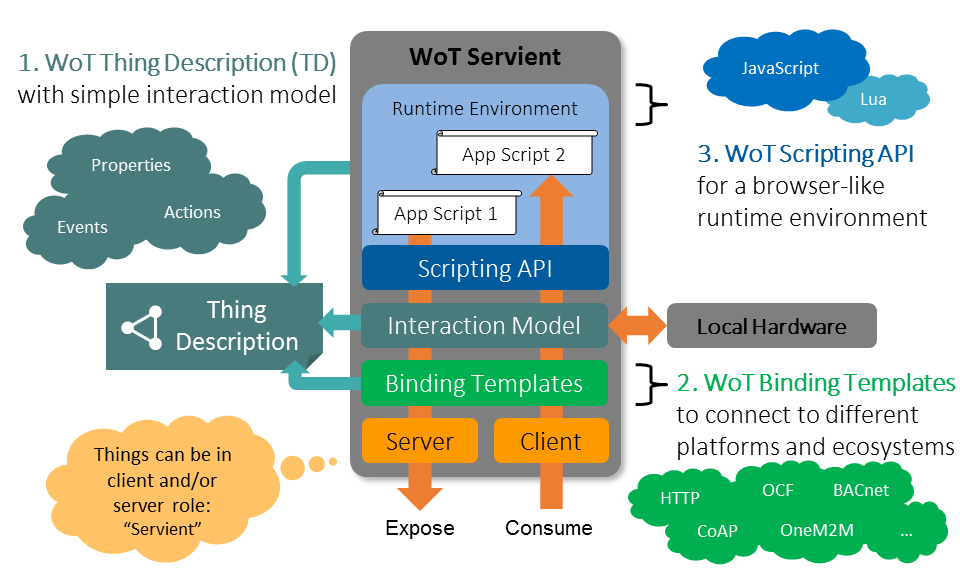
\includegraphics[width=3.3in]{figures/wot-servient.png}
\caption{WoT Servient architecture}
\label{fig-fservient}
\end{figure}




\subsection{Threat Model}
%\textsf{A basic intro to to the WoT threat model~\cite{Wot2017sec}.}

Due to the large diversity of devices,
use cases,
deployment scenarios 
and requirements for WoT Things,
it is impossible to define a single WoT threat model
that would fit every case.
Instead we have created an overall WoT threat model
\emph{framework}~\cite{Wot2017sec} 
that can be adjusted by OEMs or other WoT system users or providers
based on their concrete security requirements.

%The WoT threat model defines the following key WoT Assets that are important from security point of view:	\textit{Thing Description}, \textit{Thing User Data} (any user data transferred via WoT network, such as video streams, sensor data etc.), \textit{Thing Provider Data} (WoT application scripts and their configuration data), \textit{WoT Basic Security Metadata} (all provisioned security medatada), \textit{WoT Controlled Environment} (physical environment that can be affected by WoT Things), \textit{WoT Thing and Infrastructure Resources} (resources of devices providing WoT Things and overall WoT network) and \textit{WoT Behavior Metrics} (all indirectly transmitted information).
%Some of these assets might be absent and/or have different trust model (i.e who should have a legitimate access and to what extent) depending on deployment scenario. 

The threat model defines security-relevant WoT assets 
and a set of threats on these assets.
Threats can be in or out of scope based on the deployment scenario,
security objectives, acceptable risks, and other factors.
For example,
in a smart home scenario involving WoT Things that record audio/video
information, privacy would usually be considered important and 
therefore this scenario would have high confidentiality requirements.
On another hand,
in an industry automation scenario involving WoT Things that 
control some safety-critical infrastructure,
confidentiality might not be the highest priority.
Instead, in an industrial setting, service availability
and protection of the environment controlled by the Thing 
may be of topmost importance.

Deploying the WoT in a distributed system brings additional complexity 
to the WoT Threat Model and the choice of relevant security mitigations.
In particular one cannot rely on single standard communication infrastructure 
and protocol 
(like HTTPS) to provide an end-to-end security between all communicating
parties.
Instead WoT needs to support multiple security mechanisms 
(potentially nested or interdependent) 
that can be combined into single end-to-end security solution.  
 


\subsection{Typical Deployment Scenario}
Figure~\ref{fig-wot-scenario} presents a typical WoT deployment scenario. 
A WoT Thing device together with a WoT Servient are located on a 
local network and accessed through a forwarding proxy. 
A WoT Client (which may in general be located either outside of the local network,
as shown, but in many use cases may also be inside) wants to 
perform interactions on the WoT Thing and WoT Servient.
The available interactions are given in corresponding Thing Descriptions.
There are various ways Thing Descriptions provided by WoT Things
could be made available to WoT Clients.
In this case, the Thing Descriptions are 
uploaded by the WoT Thing and WoT Servient to a Thing Directory.
A Thing Directory is a service which can be accessed by Clients
to search for WoT Things it can communicate with.
In order to do this the WoT Client first needs to issue a 
discovery query to the Thing Directory.
Thing Directories can support semantic search capabilities, allowing
Things to be discovered based on semantic annotations. 
Access to the search capabilities of a Thing Directory should
only be provided to authorized clients, as with any web service.
Upon obtaining a Thing Description, 
the WoT Client needs to make sure it has all the necessary credentials
to authenticate to the forwarding proxy 
(assuming secure authentication on the proxy is enabled), 
the WoT Servient and in some cases even to the specific WoT Thing.
Information describing how clients need to authenticate themselves
should be provided in the obtained Thing Descriptions.  

\begin{figure*}[!t]
\centering
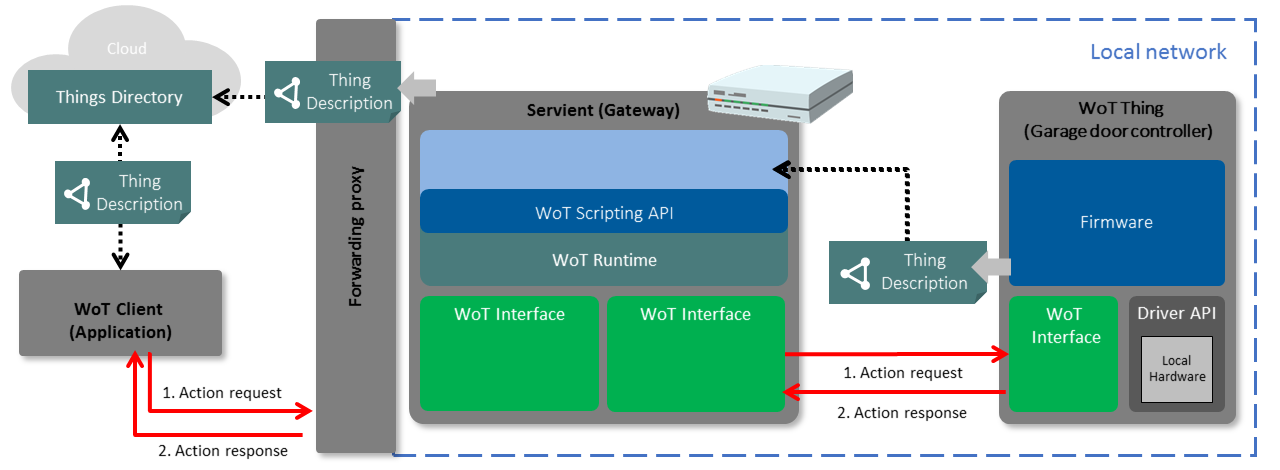
\includegraphics[width=6in]{figures/wot-scenario.png}
\caption{Typical WoT deployment scenario}
\label{fig-wot-scenario}
\end{figure*}


% Best practices in IoT that are *common* to WoT... and that we will NOT focus on
% We want to explain in particular how WoT is different
\section{Related Work}
% Some relevant prior work: 
% State-of-the-Art and Challenges for the Internet of Things Security \cite{Garcia2017a}.
% The Industrial Internet of Things Security Framework \cite{Iic2016sf}.
% IoT Security Foundation Best Practices Guidelines \cite{Iotsf2017a}.
The WoT approach applies to a wide diversity of IoT devices and use cases.
It has to take be able to support best practices in IoT security which
are however still rapidly evolving.
Recently some attempts have been made to define
best practices for IoT security.
The IETF Thing-to-Thing Research group has a RFP under development,
\emph{State-of-the-Art and Challenges for the Internet of Things 
Security}~\cite{Garcia2017a}, which includes a threat model similar to 
what we have defined for the WoT.  However, it does not consider the 
importance of protecting access to descriptive metadata.
The Industrial Internet of Things has published a comprehensive
\emph{Security Framework}~\cite{Iic2016sf}.
This is useful, but focuses on industrial use cases.
The IoT Security Foundation has published
a \textit{Best Practices Guidelines}~\cite{Iotsf2017a}
document as well.
All three documents consider various additional factors we do
not have time to go into here, such as trust management over the 
lifecycle of the device.

There are several survey papers~\cite{Iot2020,Xu2014,Fernandes2017} that attempt to describe 
the current IoT security challenges and provide suggestions for the future work in the area.





% What are some specific interesting problems/solutions that WoT brings?
\section{Risks and Opportunities}
\label{sec-risks-opportunities}

\subsection{Local Links}
Many issues arise when trying to access IoT devices
that are located on a ``local'' network,
for example behind a NAT in a Smart Home (consumer) use case,
or on a firewalled operational network in a Smart Factory
(industrial) use case.
In addition, devices may be accessible over multiple
routes and protocols, raising the problem of unique identification.

When one hears the term ``Web of Things'' the
assumption is that HTTP will be used to
access IoT devices. 
While leveraging web standards was one of the 
original goals of the Web of Things concept~\cite{Ostermaier2010},
the current WoT draft supports other choices as well,
such as CoAP and MQTT.
However, use of HTTP conveniently
allows Things acting as web servers to be accessed directly
from web browsers to provide human user interfaces via HTML.  
To provide better security, one would
naturally want to use HTTPS rather than HTTP.
Unfortunately the way HTTPS is supported in web browsers has
been designed for globally accessible web sites, not devices
behind NATs that may or may not have a globally accessible
address and may not even be continously connected to the internet.
In particular, certificate revocation checks as currently 
implemented in web browsers will not work if
the network both devices are on is not connected to the internet
(for example, if an \textit{ad hoc} network is used, with the device acting as
an access point) and certificates will not generally be able 
to tie the identity of a device to a particular unique URL. 

Both of these problems can be avoided by using a cloud proxy
or mirror (digital twin) for the device.
In that case a server
in the cloud is used as an intermediary.
Unfortunately,
this requires an active internet connection even to use 
local devices, has relatively high latency, and is
bandwidth-inefficient.
Various mechanisms have been explored to deal with this issue~\cite{httpslocal2017}
but no generally accepted solution has been adopted.
Therefore a metadata standard needs to be able to deal with a variety
of approaches.

% Other secure protocols, like CoAPS, 
% do not have the same assumptions as HTTPS and can be used
% more easily in an segmented network.
% As noted above the WoT, despite its name, can also work with these standards.
The issues noted above are not directly relevant if humans do not need
to communicate directly with a Thing using a web browser.  
In machine-to-machine (M2M) use cases
we have more flexibility in how we establish trust and validate connections.

Even for M2M use cases there is another issue: the URLs
used to access the same device can vary depending on whether the
device is accessible on the local network or should be accessed
via a global URL (either via NAT port forwarding, a proxy, or
a digital twin).
A Thing Description can include multiple links
for each interaction,
so in theory both local and global links
can be included in a single Thing Description.
However,
a user of a Thing has no easy way to tell if it is on
the same local network as another target Thing,
and if not, the ``local'' links won't work.
Another
approach would be for a trusted and authenticated
Thing Directory to return a modified
Thing Description with local links to clients that it (somehow) knows 
are on the same local network.
%However a mechanism is needed to ensure only
%authenticated and trusted Thing Directories can do such redirection,
%since redirection raises the possibility
%of a malicious Thing Directory, or a network attacker spoofing a
%Thing Directory, redirecting clients to fake devices.

A related issue is that of unique identity.
The linked data approach used to support semantics in the WoT
is based on the use of unique URIs to identify entities.
However, if a Thing can be accessed using multiple URLs then
these cannot be used to uniquely identify a Thing---or at least, not all of them. 
Currently under discussion are ways in
which unique identifiers can be added to Thing Descriptions,
separate from the links used for interactions.
These unique identifiers could be based on URI schemes such as UUIDs and DOIs.
Use of unique identifiers also raises (or perhaps only highlights) privacy considerations.
Potential privacy mitigations include limiting access to the unique identifiers in
Thing Descriptions to authorized users and
allowing unique identifiers to be reset as needed,
for example upon ownership transfer.


\subsection{Vulnerability Scanning}
Thing Descriptions are meant to enable easier discovery and use of 
devices.  The flip side of this is that it may also become easier
for attackers to discover vulnerable devices, or to infer private information
simply from the type of devices available.

The first line of defense is to protect access to discovery services such
as Thing Directories.  If Thing Directories can only be accessed by authorized
users, a number of types of attacks become more difficult.  Since a Thing
Directory is simply a web service, it can be protected with normal web service
authorization and security mechanisms.  
However, a given WoT implementation may provide other means of 
discovery, such as broadcast responses or extended DNS entries.
These may not be as easy to protect.
In order to support a protected Thing Directory
a protected onboarding process is needed to associate devices with a given
Thing Directory.
A mechanism is also needed to provide authorized entities with appropriate
credentials to access the Thing Directory.

Assuming an attacker can access Thing Descriptions, however, they may be
able to exploit them in various ways.  First, they could try to analyze the 
available interactions themselves for known vulnerabilities.  While the 
Thing Descriptions intentionally omit information about the software stack
providing the service, an attacker may be able to use fingerprinting to
associate a particular Thing Description with a particular device or software stack
with known vulnerabilities.  The vulnerabilities may not even be over the network;
for example, an attacker may scan for ``smart locks'' that can be defeated
with known physical attacks.
The flip side of this, however, is that a System Maintainer can apply the same
tools to scan for devices with vulnerabilities, in order to identify devices
at risk so that mitigations can be put in place (such as scheduling updates to
a device's firmware, or enhancing the physical protection of a device).
Unlike a malicious attacker, the System Maintainer also has the advantage that
they can legitimately access \emph{all} Thing Descriptions in a system.

Even if an attacker cannot determine vulnerabilities, they may still be able
to determine personal information about a user by the kinds of devices they
have installed.  For example, knowing that someone has a baby monitor lets you
infer that they probably have a young child.
Semantic tags make this information explicit but even without tagging,
fingerprinting may be able to associate a set of interactions with
a specific class of devices.  The mitigation of this kind of attack is to
protect the Thing Descriptions themselves and make them available
\emph{only} to authorized users.


\subsection{Endpoint Adaptation}
% \textsf{End-to-end secure adaptation by pushing payload transformation to endpoints.}
In a typical multistandard IoT system,
bridges may be needed to connect devices
conforming to different standards.
For example,
to connect to an AllJoyn device from a controller
designed to connect to OCF devices, an OCF-to-AllJoyn bridge
may be needed to translate both the protocol and the payload.
In general, multiple bridges could be involved: the
apparent AllJoyn device could in fact be a oneM2M device
being made available over yet another bridge.

Unfortunately bridges introduce a potential security vulnerability.
If the bridge devices can be compromised,
an attacker can have full access to the
data being carried to and from the device can can stage a 
variety of attacks: 
modifying or deleting data,
injecting false data and events,
or privacy invasion.

The WoT enables a way around this problem using endpoint 
end-to-end payload adaption.
This is complementary to but distinct from object security~\cite{Mattsson2014}.

Rather than adapting payloads in a point-to-point fashion,
adaptation should take place at one of the endpoints, ideally the
one with greater capability.  The endpoint doing the adaptation should
look at the metadata for the target endpoint, adapt its payload for that
target, and then use end-to-end encrypted communication:
either end-to-end transport security, object security, or both.

However, if multiple transport protocols are used, such as a 
combination of HTTP/TLS and CoAP/DTLS, bridging those protocols
may create another compromise possibility.  A mechanism supporting
object security such as JOSE~\cite{Jose2017} should then be used
in combination with endpoint adaptation, but of course for this to
work the target (typically constrained) endpoint needs to support it. 
Object security also supports secure state caching in the cloud or gateways,
an important consideration for devices that may need a digital
twin to handle transactions for them while they are in standby,
conserving battery, or otherwise offline.



\subsection{Secure Discovery}
One of the benefits provided by the WoT approach is to
enable the use of powerful semantic searches during discovery.
However, this introduces several issues related to security.

First of all, semantic searches can be abused to create DoS attacks.
If arbitrary SPARQL endpoints are provided by Thing Directory
services, semantic searches can be specified
that can consume large amounts of resources,
rendering the Thing Directories unavailable to other users.
This can be mitigated by either limiting the power of searches
that can be specified, or by limiting the processing
power that can be used in a specific search.

In the first approach, rather than providing a full
SPARQL endpoint, a directory service may provide a more specialized
search interface that only allows searches for a conjunction of terms
and does not allow, for instance, use of arbitrary inference rules
or use of other SPARQL endpoints in a federated search.
However, by limiting the power
of the searches that may be specified, we are also limiting the
potential benefit.

The second approach to mitigate DoS attacks 
is to use an architecture for the 
search engine that can enforce resource quotas on individual queries.
For example, each search could be spawned in a new process and Linux
process limits could be used to enforce processing quotas. In addition,
the number of searches that can be processed at the same time would
have to be limited to avoid creating too many processes.
If either limit is exceeded the server would return an appropriate
error code.  If the query processing quota is exceeded, the client
would have to reformulate their query.  If the server is too busy,
the client would have to retry the query later.

Of course creating a new process for each search would be expensive,
so ideally the search engine itself would have lighter-weight
mechanisms to track resource consumption and enforce quotas.

There is another class of risks with semantic searches: 
inferencing. 
By their nature, semantic searches can infer information that is
not explicitly present in the database.
It is possible that an attacker could use this capability
to invade someone's privacy.  For example, they could infer
personal information (e.g. marital status) from the ownership
of certain combinations of devices (e.g. multiple toothbrushes).
While it is difficult to prevent inference attacks in general,
we should at least design semantic search engines to not use 
data for inference that would not be directly available to the
person posing the query in the first place~\cite{Thura2005a,Xia2014a}.  
As with the other class of risks we mentioned,
mitigation requires restricting the distribution of Thing Description
data to authorized users only.


\subsection{Enabling Distributed Security}
Many things must be taken into account when choosing what metadata to include in a TD: 
deployment scenarios and configurations, 
underlying networking protocols and their security mechanisms, 
overall scalability, system security priorities, and so on.
Security metadata should support security mechanisms in current use by both 
web services~\cite{openapi2018} and IoT systems~\cite{ace2017,ocf2017}.
The TD should be extensible enough to support emerging capabilities
related to security, for
example for micropayments~\cite{interledger2017} or smart contracts.

A data packet in a IoT system can go over many intermediate entities,
including gateways and proxies.
Some of these entities might need to perform authentication 
and authorization of the requester. 
Security metadata in a TD can indicate
what types of authentication are required by each entity
and how to obtain authorizations.
The metadata can also specify roles and security policies,
and perhaps different ones for different interactions.

Consider the deployment scenario in Figure~\ref{fig-wot-scenario}.
Suppose the forwarding proxy requires authentication of any request before passing it to the local network.
Additionally assume that the WoT gateway performs its own authentication.
Both of these authentication methods and 
associated information can be specified in the TD 
that the WoT Client receives from the Thing Directory.
Users of a WoT Thing may also have different roles with different access rights,
and may want to delegate some rights to others on a permanent or temporary basis.
%For example, a homeowner may have the ability to open and close a garage door and
%also query its current state and its power consumption.  The same homeowner may
%however want to allow a security service to monitor the state of the door in order
%to flag anomalies (such as the door opening when no one with access rights is
%at home). The homeowner may also want to be able to temporarily delegate rights
%to open the door to visitors.
%Yet another role is that of system administrator, who would need the ability to
%update the firmware on the device; such access would obviously be unwise to provide
%to visitors.

The WoT gateway can perform the authentication and access control to WoT Clients 
in a number of ways depending on what standards the target devices support.
For example, the OCF Security Specification~\cite{ocf2017}, which is one possible
system whose devices can be described by WoT TDs, 
supports a number of ways IoT devices can perform authentication based on 
either symmetrical or asymmetrical credentials (including certificates),
and also supports access control lists.
%However, provisioning credentials in advance 
%is not ideal for a distributed network such as the WoT is intended to support.
In general, we want to support fine-grained role-based access control
so that access rights can be granted (and revoked) without having to directly
update the state of devices.
Token-based authentication mechanisms
such as Bearer or Proof-of-Possession tokens~\cite{ace2017} can be used for this.
Token-based authentication allows  
a client to dynamically request a token from a remotely 
located authorization server and present it for 
authentication as needed.
This method has its own risks and limitations;
bearer tokens, for example, need to be protected from interception.
% However, token-based authentication can be combined with access control 
% lists to provide fine-grained role-based access policies.

Generalizing the above example, 
there might be $N$ sets of fully independent security metadata
necessary in a Thing Description.
Moreover, when a Thing Description is composed, 
these sets can be provided by separate entities: 
a gateway might only specify the security metadata for accessing interactions defined in a TD,
while the forwarding proxy adds the metadata required for successful authentication of incoming requests.
This means that there has to be a way to limit what security metadata 
is allowed to be provided by what entity.
Also, it must be possible for the WoT client to verify the overall integrity of the resulting TD. 
 


\section{Conclusion}
We have given a summary of the W3C Web of Things draft
standard, with a focus on the Thing Description.
The Thing Description provides a descriptive approach to 
interoperability, which contrasts with the prescriptive
approach of most other standards.
While a prescriptive approach is useful, for example to
enforce minimum security requirements,
a descriptive approach can support brownfield devices
and can also make it easier to integrate devices that
conform to different prescriptive standards.

However, beyond the basic issue of integrating devices
with different levels and mechanisms for security,
which will arise with any multistandard IoT system,
the use of descriptive metadata raises several
new security risks and opportunities.  

With the goal of starting discussion,
we have presented five such problems: 
security over local and multiple links,
multidevice vulnerability analysis,
end-to-end security enabling,
secure discovery for semantic interoperability,
and (potentially decentralized) security mechanism enabling.


\section*{Acknowledgment}
The security and threat model presented here was developed 
in the W3C Web of Thing WG as part of the 
\textit{Web of Things (WoT) Security and Privacy Considerations} 
document~\cite{Wot2017sec}. Please see the associated github site
for a list of additional contributors.
Barry Leiba provided feedback on an early draft.


\bibliographystyle{IEEEtranS}
\bibliography{refs}
\end{document}


